% FM-Empfänger: Blockschema mit Signalverlauf nach jeder Stufe (Daten: fm_empf_*.dat, x in cm)
\resizebox{\linewidth}{!}{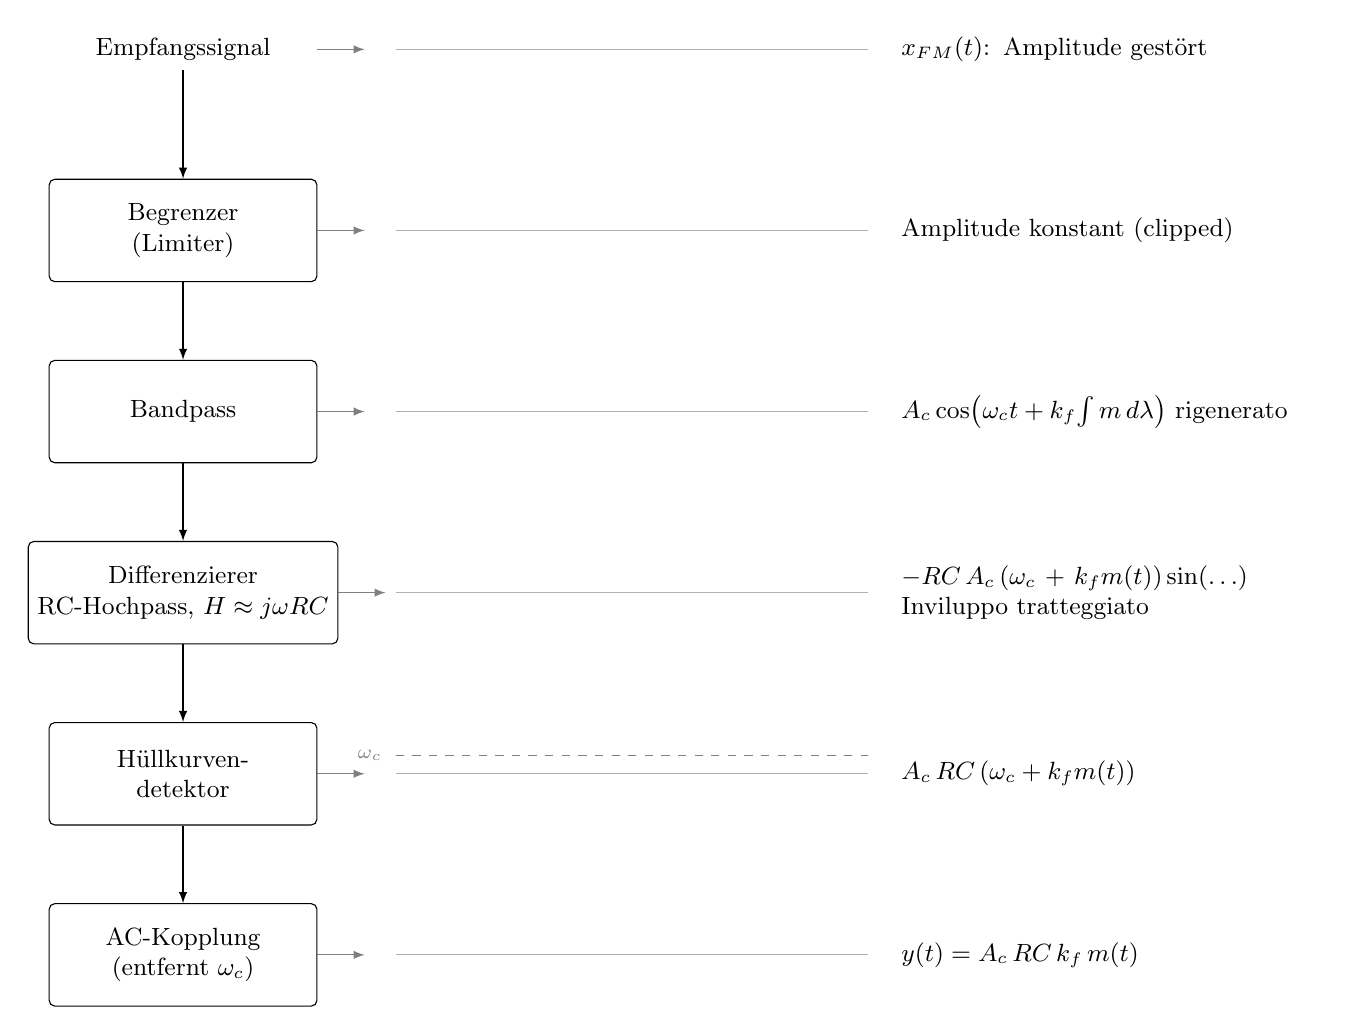
\begin{tikzpicture}[blk/.style={draw,rounded corners=2pt,minimum width=3.4cm,minimum height=1.3cm,align=center,font=\small},frm/.style={font=\small,anchor=west,text width=5.2cm,align=left}]
\def\D{chapters/06_amplitudenmodulation/figures/}
\def\P{2.3}
\node[align=center,font=\small,minimum width=3.4cm] (b0) at (1.9,0) {Empfangssignal};
\node[blk] (b1) at (1.9,-\P) {Begrenzer\\ (Limiter)};
\node[blk] (b2) at (1.9,-2*\P) {Bandpass};
\node[blk] (b3) at (1.9,-3*\P) {Differenzierer\\ RC-Hochpass, $H\approx j\omega RC$};
\node[blk] (b4) at (1.9,-4*\P) {Hüllkurven-\\detektor};
\node[blk] (b5) at (1.9,-5*\P) {AC-Kopplung\\ (entfernt $\omega_c$)};
\foreach \i/\j in {0/1,1/2,2/3,3/4,4/5}{\draw[-latex] (b\i.south) -- (b\j.north);}
\foreach \i in {0,...,5}{
  \draw[-latex,gray] (b\i.east) -- ++(0.6,0);
  \draw[gray!60,thin] (4.6,-\i*\P) -- (10.6,-\i*\P);
}
\begin{scope}[shift={(4.6,0)}]\draw[blue!60!black,thick] plot file{\D fm_empf_0.dat};\end{scope}
\begin{scope}[shift={(4.6,-\P)}]\draw[blue!60!black,thick] plot file{\D fm_empf_1.dat};\end{scope}
\begin{scope}[shift={(4.6,-2*\P)}]\draw[blue!60!black,thick] plot file{\D fm_empf_2.dat};\end{scope}
\begin{scope}[shift={(4.6,-3*\P)}]
  \draw[gray,dashed] plot file{\D fm_empf_3e.dat};
  \draw[gray,dashed] plot file{\D fm_empf_3n.dat};
  \draw[red!70!black,thick] plot file{\D fm_empf_3.dat};
\end{scope}
\begin{scope}[shift={(4.6,-4*\P)}]
  \draw[gray,dashed] (0,0.233) -- (6,0.233);
  \draw[green!40!black,very thick] plot file{\D fm_empf_4.dat};
\end{scope}
\begin{scope}[shift={(4.6,-5*\P)}]\draw[violet!80!black,very thick] plot file{\D fm_empf_5.dat};\end{scope}
\node[font=\scriptsize,gray,anchor=east] at (4.55,-4*\P+0.233) {$\omega_c$};
\node[frm] at (10.9,0) {$x_{FM}(t)$: Amplitude gestört};
\node[frm] at (10.9,-\P) {Amplitude konstant (clipped)};
\node[frm] at (10.9,-2*\P) {$A_c\cos\!\big(\omega_c t+k_f\!\int m\,d\lambda\big)$ rigenerato};
\node[frm] at (10.9,-3*\P) {$-RC\,A_c\,(\omega_c+k_f m(t))\sin(\dots)$ Inviluppo tratteggiato};
\node[frm] at (10.9,-4*\P) {$A_c\,RC\,(\omega_c+k_f m(t))$};
\node[frm] at (10.9,-5*\P) {$y(t)=A_c\,RC\,k_f\,m(t)$};
\end{tikzpicture}}
